% MobiWac 2026 talk -- Paris, Monday 2026-10-26, 8:30, Session 1 (first talk of the symposium).
% 30 min slot INCLUDING Q&A. Main track follows ../PLANO_APRESENTACAO.md §4 **v2** (12 slides,
% ~14:50, commit 138f97a9); backup = §5 (B1-B10).
%
% OWNERSHIP (one owner per file, the rule from the defense):
%   ../PLANO_APRESENTACAO.md  -> session `mobiwac` (content: what goes on each slide, and the talk)
%   this file                 -> session `mobiwac-ppt` (the only hand that edits the .tex)
% Change the plan first, then propagate here. Locate frames by title, never by line number.
%
% NUMBERS: every number on screen comes from ../../CAMERA_READY.md §3 (v18, joint-best) or from the
% camera-ready text in ../../src/. The defense deck is NOT a source. ⛔ PLANO §2.2 lists the v17
% values that must never appear here (incl. the km near-miss metric).
%
% BUILD: `make all` (xelatex x3 + bibtex). NEVER pdflatex -- the title page renders blank.
% Style law inherited from articles/dissertacao/presentation/{HANDOFF,BOAS_PRATICAS_SLIDES}.md:
% no \scriptsize for content, a frame body never opens with "{" (the `\vspace{0pt}` guards),
% canary + render after each build. Em-dash only as label separator / subtitle (HANDOFF §4f).
% American English (paper GLOSSARY): "neighborhood", not "neighbourhood".

\documentclass{beamer}
\usepackage[net,green]{nesped}
\usepackage[english]{babel}
\graphicspath{{img/}{figures/}}
\usepackage{booktabs}
\usetikzlibrary{arrows.meta,calc}

\title[Next Category and Region of a Visit]{Predicting the Next Category and Region of a Visit}
\subtitle{A Check-in-Level Multi-Task Study on Mobility Data}
% Names as in the camera-ready (src/main.tex). The program lists "Germano dos Santos".
\author{Vitor Hugo de Oliveira Silva \and Germano Barcelos dos Santos \and Fabrício Aguiar Silva}
\institute[UFV]{NESPeD-LAB $\cdot$ Universidade Federal de Viçosa, Brazil}
\date{MobiWac 2026 $\cdot$ Paris $\cdot$ October 26, 2026}

\setlength{\columnsep}{6mm}

% Verdict cell colors (S7, B10): green = outperforms the dedicated model; grey = inside the bound.
\newcommand{\win}[1]{\textbf{\color{primaryshade}#1}}
\newcommand{\flatc}[1]{{\color{black!55}#1}}

\begin{document}

% ============================================================
% S1 · Title (PLANO v2 §4 S1, 20 s)
% ============================================================
\titleframe{
    \titlelogo{img/logo-nesped.png}
    \titlelogo{img/logo-ufv.png}
}

% ============================================================
\section{Question}
% ============================================================

% S2 · One person's day, and the question (PLANO v2 §4 S2, 130 s). The script is in the plan,
% nearly word for word -- it is NOT duplicated here (the plan owns the talk).
% The figure is drawn here (no plate existed). It is SCHEMATIC: the tract mesh is a jittered
% lattice with a fixed seed, not a real map, and the dots are not a real user.
% ⚠ "Region" is DEFINED on this slide (Fable F3). ⚠ Handover is an ANALOGY of scale, never a
% claim (Fable F2; src/sections/04_method.tex, "a census tract is a neighborhood, not a radio cell").
\begin{frame}{One person's day, and the question}
    \vspace{0pt}% guard
    \centering
    \begin{tikzpicture}[x=1mm,y=1mm,
            ci/.style={circle,fill=secondary,inner sep=0pt,minimum size=2.1mm},
            hop/.style={-{Stealth[length=1.6mm]},secondary,line width=0.6pt},
            lab/.style={font=\footnotesize\itshape,text=black!70}]
        % --- the tract mesh (schematic): jittered lattice, fixed seed ---
        \pgfmathsetseed{11}
        \foreach \i in {0,...,12}{
            \foreach \j in {0,...,4}{
                \pgfmathsetmacro{\dx}{rand*2.2}
                \pgfmathsetmacro{\dy}{rand*1.8}
                \coordinate (m-\i-\j) at ({\i*9+\dx},{\j*8.5+\dy});
            }
        }
        \begin{scope}
            \clip[rounded corners=4mm] (-1,-1) rectangle (109,35);
            \fill[black!3] (-1,-1) rectangle (109,35);
            % the unknown next tract
            \fill[alert!18] (m-10-2) -- (m-11-2) -- (m-11-3) -- (m-10-3) -- cycle;
            \foreach \i in {0,...,11}{
                \pgfmathtruncatemacro{\ni}{\i+1}
                \foreach \j in {0,...,4}{
                    \draw[primary!40,line width=0.5pt] (m-\i-\j) -- (m-\ni-\j);
                }
            }
            \foreach \i in {0,...,12}{
                \foreach \j in {0,...,3}{
                    \pgfmathtruncatemacro{\nj}{\j+1}
                    \draw[primary!40,line width=0.5pt] (m-\i-\j) -- (m-\i-\nj);
                }
            }
        \end{scope}
        \draw[black!35,rounded corners=4mm,line width=0.5pt] (-1,-1) rectangle (109,35);
        % --- nine check-ins ---
        \node[ci] (v1) at (8,8)   {};
        \node[ci] (v2) at (20,5)  {};
        \node[ci] (v3) at (31,12) {};
        \node[ci] (v4) at (27,24) {};
        \node[ci] (v5) at (41,28) {};
        \node[ci] (v6) at (52,19) {};
        \node[ci] (v7) at (63,9)  {};
        \node[ci] (v8) at (75,15) {};
        \node[ci] (v9) at (84,24) {};
        \foreach \a/\b in {v1/v2,v2/v3,v3/v4,v4/v5,v5/v6,v6/v7,v7/v8,v8/v9}{
            \draw[hop] (\a) -- (\b);
        }
        \node[lab,above=0.6mm] at (v1) {coffee};
        \node[lab,below=0.6mm] at (v2) {gym};
        \node[lab,right=0.6mm] at (v3) {office};
        \node[lab,above=0.6mm] at (v5) {lunch};
        % --- the tenth: the question ---
        \coordinate (qc) at ($(m-10-2)!0.5!(m-11-3)$);
        \node[font=\Large\bfseries,text=alert] (q) at (qc) {?};
        \draw[-{Stealth[length=1.6mm]},alert,line width=0.8pt,dashed] (v9) -- (q);
    \end{tikzpicture}

    \vspace{1.5mm}
    \begin{columns}[T,onlytextwidth]
        \begin{column}{0.465\textwidth}
            \begin{block}{What kind of place?}
                \footnotesize \textbf{Next category}: one of 7 types, such as food, shopping,
                nightlife.
            \end{block}
        \end{column}
        \hfill
        \begin{column}{0.465\textwidth}
            \begin{block}{Which neighborhood?}
                \footnotesize \textbf{Next region}: its census tract, 520 to 8,501 per dataset
                (Istanbul: \emph{mahalle}).
            \end{block}
        \end{column}
    \end{columns}

    \vspace{0.5mm}
    {\footnotesize A tract is a neighborhood, \alert{not a radio cell}: we claim nothing about
    cells or handover.\par}
\end{frame}

% ============================================================
\section{Representation}
% ============================================================

% S3 · Check2HGI (PLANO v2 §4 S3, 100 s) -- the defense's two frames fused (plate + "What each
% visit contributes"). ⚠ Keep the forward-only clause: limit 3 of the paper and the B4 anchor.
\begin{frame}{Check2HGI: a fourth level below the place}\label{fr:visit-past}
    \vspace{0pt}% guard
    \vfill
    \noindent\makebox[\textwidth]{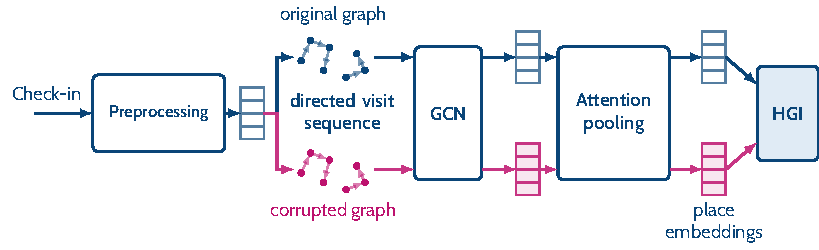
\includegraphics{c2h_deep}}
    \vfill
    {\footnotesize
    \leftskip=1.2em \parindent=-1.2em
    \textcolor{primary}{$\blacktriangleright$}~\textbf{Each visit carries} its place's category, the
    hour and day of week, and four elapsed-time values $\to$ one \textbf{64-d} vector per visit.\par
    \smallskip
    \textcolor{alert}{$\blacktriangleright$}~\textbf{Built from the past alone}: edges between
    consecutive visits run forward in time only, and the graph never sees the next category or
    region.\par}
    \leftskip=0pt \parindent=0pt
\end{frame}

% S4 · Result 1 (PLANO v2 §4 S4, 115 s) -- table reused from the defense deck (cell-by-cell vs
% CAMERA_READY §3.3). CORRECTED 2026-10-03 (author: the deck shows the corrected numbers): Istanbul
% place cell is the PAIRED re-run, 32.54 / +2.81 (docs/results/closing_data/v18/istanbul_pair/), not the
% published unpaired 29.07 / +6.29. Dissertation B.5 rows 22-28. The feature-concatenation control is SPOKEN here (plan) and has its own B9.
\begin{frame}{Result 1: the representation, at every dataset}
    \framesubtitle{Next category, single-task model, seed 0 --- only the input changes}
    \begin{center}
        \small
        \setlength{\tabcolsep}{9pt}
        \begin{tabular}{@{}lrrr@{}}
            \toprule
            \textbf{Dataset} & \textbf{Check-in level} & \textbf{Place level} & \textbf{$\Delta$} \\
            \midrule
            AL       & \textbf{30.77} $\pm$1.16 & 29.15 $\pm$0.84 & $+1.62$ \\
            AZ       & \textbf{34.51} $\pm$1.15 & 31.93 $\pm$1.08 & $+2.58$ \\
            Istanbul & \textbf{35.35} $\pm$0.89 & 32.54 $\pm$1.03 & $+2.81$ \\
            FL       & \textbf{37.36} $\pm$0.42 & 37.13 $\pm$0.41 & $+0.23$ \\
            CA       & \textbf{35.62} $\pm$0.47 & 34.74 $\pm$0.41 & $+0.88$ \\
            TX       & \textbf{36.32} $\pm$0.51 & 35.33 $\pm$0.48 & $+0.99$ \\
            \bottomrule
        \end{tabular}\par
        \smallskip
        {\footnotesize macro-F1; five matched folds, $\pm$ is the fold sd.\par}
    \end{center}

    {\footnotesize
    \textbf{Larger at the three smaller datasets} ($+1.6$ to $+2.8$), under one point at the three
    largest. A paired test separates the two at five of six; \alert{not at Florida}.\par}
\end{frame}

% ============================================================
\section{Model}
% ============================================================

% S5 · Why sharing is not free, and the model (PLANO v2.2 §4 S5, 75 s; author 2026-10-01 via
% `mobiwac`). Reading order INVERTED: first the risk, then the figure as the answer to it.
% ⚠ "multi-task learning" is never a concept to define here (plan rule): the risk is said in the
% room's own words. No block counts, no widths.
% ⚠ The figure says "semantic/spatial stream" (it is Fig. 2 of the paper); say it once aloud.
\begin{frame}{Why sharing is not free, and the model}
    \vspace{0pt}% guard
    \begin{columns}[c,onlytextwidth]
        \begin{column}{0.60\textwidth}
            \centering
            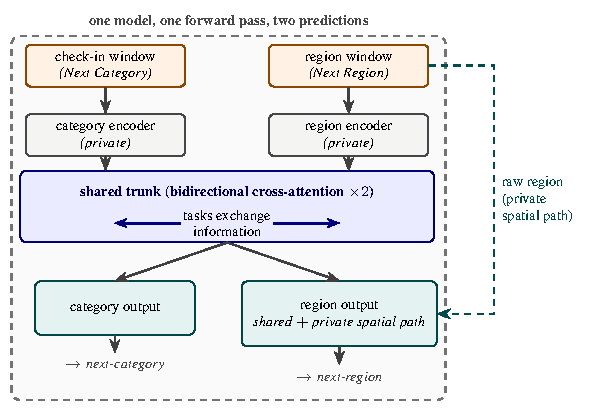
\includegraphics[width=\linewidth]{fig2_model_slides}
        \end{column}
        \hfill
        \begin{column}{0.37\textwidth}
            \small
            \textbf{\color{alertshade}The risk}\par\smallskip
            Parameters in the middle serve \textbf{both jobs at once}, and can settle on a
            compromise \alert{worse for each}.\par\vspace{4mm}
            \textbf{\color{primaryshade}The answer}\par\smallskip
            A \textbf{shared trunk}, where each task reads the other's context; and a
            \textbf{private spatial path} for region that category never touches.\par\vspace{4mm}
            \alert{\textbf{The private path is the architecture admitting the risk.}}\par
        \end{column}
    \end{columns}
\end{frame}

% S6 · How it was measured (PLANO v2 §4 S6, 90 s) -- the defense's four protocol frames in one.
% ⚠ The sentence that is never cut: the margin written before any result was seen.
% The "Scored" row is NOT in the plan's four lines: added so that Acc@10 is defined before S7
% reads it (flagged to `mobiwac`, 2026-09-30).
\begin{frame}{How it was measured}
    \vspace{0pt}% guard
    \small
    \setlength{\tabcolsep}{6pt}
    \renewcommand{\arraystretch}{1.5}
    \begin{tabular}{@{}p{0.2\textwidth}p{0.74\textwidth}@{}}
        \toprule
        \textbf{Regions}  & census tracts, \textbf{520} (Istanbul) to \textbf{8,501} (California) \\
        \textbf{Split}    & by user: the visits of a test user \textbf{never appear in training} \\
        \textbf{Scored}   & category: \textbf{macro-F1} $\cdot$ region: \textbf{Acc@10}, is the true
                            region in the top ten? \\
        \textbf{Repeated} & \textbf{20 trained models} per configuration (4 seeds $\times$ 5 folds) \\
        \textbf{Decided}  & what counts as ``not worse'': \textbf{2 points},
                            \alert{written down before any result was seen} \\
        \bottomrule
    \end{tabular}
\end{frame}

% ============================================================
\section{Results}
% ============================================================

% S7 · One model, two answers: what it costs (PLANO v2 §4 S7, 100 s).
% Only Dedicated vs Joint, no CI on screen (CIs -> B10). Values: CAMERA_READY §3.1/§3.2.
% ⚠ The Δ column is the PAIRED difference (mean over the four seeds), the paper's own number. It is
% NOT always the difference of the two rounded columns (AL reg -0.87 vs 70.12-69.24; FL, TX, AL cat
% likewise, CAMERA_READY §7, item 6). The footnote says so on screen, because subtracting the columns is
% the first thing a careful listener does.
% Spoken with the numbers (plan): the joint model is also the larger one; the pairing of the two
% wins with the two largest region counts is an observation, not a law.
\begin{frame}{One model, two answers: the price}
    \vspace{0pt}% guard
    \begin{center}
    \small
    \setlength{\tabcolsep}{5.5pt}
    \begin{tabular}{@{}l rrr @{\hspace{1.6em}} rrr@{}}
        \toprule
        & \multicolumn{3}{c}{\textbf{Next region} (Acc@10)}
        & \multicolumn{3}{c}{\textbf{Next category} (macro-F1)} \\
        \cmidrule(lr){2-4}\cmidrule(lr){5-7}
        & Ded. & Joint & $\Delta$ & Ded. & Joint & $\Delta$ \\
        \midrule
        Alabama    & 70.12 & 69.24 & \flatc{$-0.87$} & 30.77 & 30.59 & \flatc{$-0.19$} \\
        Arizona    & 59.48 & 59.04 & \flatc{$-0.44$} & 34.57 & 34.57 & \flatc{$-0.00$} \\
        Istanbul   & 75.16 & 75.08 & \flatc{$-0.08$} & 35.34 & 35.42 & \flatc{$+0.08$} \\
        Florida    & 76.69 & 76.54 & \flatc{$-0.16$} & 37.35 & 37.55 & \win{$+0.19$} \\
        California & 63.48 & 64.54 & \win{$+1.06$}  & 35.63 & 35.63 & \flatc{$-0.00$} \\
        Texas      & 64.94 & 66.15 & \win{$+1.21$}  & 36.33 & 36.19 & \flatc{$-0.13$} \\
        \bottomrule
    \end{tabular}
    \end{center}

    {\footnotesize
    \win{Green}: outperforms the dedicated model. \textbf{Region}: the other four are
    \alert{deficits, not ties}, all inside the 2-point margin. \textbf{Category}: within a fifth of a
    point. $\Delta$ is the paired mean over the four seeds, so it can differ from the rounded
    columns in the second decimal.\par}

    \vspace{1.5mm}
    \begin{block}{}
        \centering\small
        \textbf{The trade is a measured one and not a free substitution.}
    \end{block}
\end{frame}

% S8 · Against published systems (PLANO v2 §4 S8, 45 s) -- demoted and reduced (Fable F1).
% CORRECTED 2026-10-03: POI-RGNN FL/CA/TX = user-disjoint reimplementation (docs/results/baselines/
% faithful_poi_rgnn_*_5f_35ep_*.json), joint category margin 4.11 (TX), not 3.06.
% CORRECTED 2026-10-04: HMT-GRN column = best validation epoch, seed 0, 5 folds (docs/results/
% closing_data/v18/g5_hmt_best_epoch/, commit 82ebfe5f), not the paper's fixed epoch 50. Region margin
% 3.55 unchanged (FL vs STAN); at CA the strongest reference becomes HMT-GRN (+4.95). Footnote wording
% from PLANO v3.1 (efb94200).
% CORRECTED 2026-10-10: STAN CA/TX now 5/5 folds, 58.61 / 61.75 (docs/results/baselines/
% stan_rerun_2026-10-10/, commit b46477a6); the partial-folds mark is gone. Region margin 3.55 unchanged.
% ⚠ "At least 4.11 / 3.55" are the JOINT model's margins. The DEDICATED model is also above every
% external, with its own smaller margins (category: FL 37.35 - 33.35 = 4.00 after the correction).
% So the screen never applies one model's margin to the other (flagged to `mobiwac`, 2026-09-30).
\begin{frame}{And against published systems}
    \vspace{0pt}% guard
    {\small\setlength{\tabcolsep}{2.6pt}
    \begin{columns}[T,onlytextwidth]
    \begin{column}{0.38\textwidth}
        \centering \textbf{Next category} {\footnotesize (macro-F1)}\\[1mm]
        \begin{tabular}{@{}lrrr@{}}
            \toprule & POI-RGNN & Ded. & Joint \\ \midrule
            AL  & 23.80 & 30.77 & 30.59 \\
            AZ  & 27.64 & 34.57 & 34.57 \\
            IST & 30.12 & 35.34 & 35.42 \\
            FL  & 33.35 & 37.35 & 37.55 \\
            CA  & 30.71 & 35.63 & 35.63 \\
            TX  & 32.08 & 36.33 & 36.19 \\
            \bottomrule
        \end{tabular}
    \end{column}
    \begin{column}{0.60\textwidth}
        \centering \textbf{Next region} {\footnotesize (Acc@10)}\\[1mm]
        \begin{tabular}{@{}lrrrrr@{}}
            \toprule & HMT-GRN & ReHDM & STAN & Ded. & Joint \\ \midrule
            AL  & 63.19 & 65.38 & 60.72 & 70.12 & 69.24 \\
            AZ  & 52.11 & 53.00 & 49.86 & 59.48 & 59.04 \\
            IST & 68.06 & 69.33 & 61.86 & 75.16 & 75.08 \\
            FL  & 72.76 & 64.49 & 72.99 & 76.69 & 76.54 \\
            CA  & 59.59 & 50.26\rlap{$^\ddagger$} & 58.61 & 63.48 & 64.54 \\
            TX  & 61.39 & 48.81\rlap{$^\ddagger$} & 61.75 & 64.94 & 66.15 \\
            \bottomrule
        \end{tabular}
    \end{column}
    \end{columns}\par}

    \vfill
    {\footnotesize
    \textbf{Both our models are above every system we compared against}; the joint model by at least
    \textbf{4.11} (category) and \textbf{3.55} (region). That margin belongs mostly to the
    representation, so \alert{it is not evidence for sharing}.\par
    \smallskip
    HMT-GRN: on our windows and folds, read at its best validation epoch, the same rule as our models.
    $^\ddagger$ReHDM: its own protocol, single seed at CA/TX.\par}
\end{frame}

% S9 · What a service would receive (PLANO v2 §4 S9, 60 s) -- NEW (DA-4 recommendation (a), v2).
% Horizon: src/sections/05_setup.tex (Windows). Shortlist + caveat: 07_discussion.tex.
% ⛔ The km near-miss metric never enters (PLANO §2.2). The shortlist reading is its substitute.
\begin{frame}{What a service would receive}
    \vspace{0pt}% guard
    \begin{itemize}\setlength{\itemsep}{2.4ex}
        \item \textbf{Lead time} --- median gap from the last visit to the next: \textbf{0.4 h}
              (Florida) to \textbf{5.5 h} (Istanbul); 5 to 27\% of the targets come more than
              3 days later;
        \item \textbf{Unseen users} --- every number is on users whose visits never appeared in
              training;
        \item \textbf{A shortlist} --- 10 regions out of \textbf{8,501} contain the true next one
              \textbf{64.54\%} of the time (California); 10 of 6,553, \textbf{66.15\%} (Texas).
    \end{itemize}

    \bigskip
    \begin{block}{}
        \centering\small
        We built and evaluated no such service: this is motivation, not a measured service result.
    \end{block}
\end{frame}

% ============================================================
\section{Wrap-up}
% ============================================================

% S10 · What it costs, and four limits (PLANO v2 §4 S10, 90 s) -- fused: the cost IS limit 4.
% Paper rounding: 1.9 M (NOT the defense's 1.85 M) -- PLANO D-1.
% CORRECTED 2026-10-20: limit 1 = dissertation e32c6507 (author, 10-06): the G1 rebuild on the delivered
% protocol moved the dedicated models by at most 0.17 macro-F1 / 0.13 Acc@10 (was the old A4 0.33 / 0.29). The four limits are the PAPER's
% (07_discussion.tex), not the defense's -- PLANO D-2.
\begin{frame}{What it costs, and four limits}
    \vspace{0pt}% guard
    \small
    \begin{columns}[T,onlytextwidth]
        \begin{column}{0.36\textwidth}
            \textbf{\color{primaryshade}THE COST}\par\medskip
            Parameters, joint vs \textbf{the two dedicated models combined}:\par\medskip
            \begin{tabular}{@{}l@{\ \ }r@{\ vs\ }r@{}}
                AL & 4.2 M & 1.9 M \\
                CA & 5.2 M & 2.8 M
            \end{tabular}\par\medskip
            What one model gives is \alert{operational}: one artifact to train, version and
            deploy; one pass, two answers.
        \end{column}
        \hfill
        \begin{column}{0.60\textwidth}
            \textbf{\color{alertshade}FOUR LIMITS}\par\medskip
            \begin{enumerate}\setlength{\itemsep}{1.4ex}
                \item Representation trained \textbf{once over all users}; a per-fold rebuild
                      moved the dedicated models by at most 0.17 macro-F1 and 0.13 Acc@10;
                \item Epoch selection reads the scored fold: \textbf{absolute scores are
                      optimistic}; joint vs dedicated is affected far less;
                \item Each visit reads \textbf{only the visits before it}
                      (slide~\ref{fr:visit-past});
                \item The joint model is \textbf{larger}: its region result may come from
                      \alert{size rather than sharing}.
            \end{enumerate}
        \end{column}
    \end{columns}
\end{frame}

% S11 · Conclusion (PLANO v2 §4 S11, 60 s) -- the CONCLUSION's words (08_conclusion.tex), not the
% abstract's "a cost bounded on both axes" (Fable F9).
\begin{frame}{Conclusion}
    \vspace{0pt}% guard
    \begin{itemize}\setlength{\itemsep}{2.6ex}
        \item The evidence \textbf{does not attribute the outcome to sharing alone}: on category, the
              representation moves the score more than the choice between one model and two;
        \item \textbf{One saved model reads both answers}: above the dedicated model on region at
              Texas and California, within the 2-point margin elsewhere;
        \item These results \alert{do not mean that multi-task learning helps automatically}.
    \end{itemize}

    \bigskip
    \begin{alertblock}{}
        \centering\small
        What a user will do next \textbf{and} where, in a single forward pass instead of two.
    \end{alertblock}
\end{frame}

% S12 · Reproducibility and acknowledgments (PLANO v2 §4 S12, 30 s) -- stays up during Q&A.
\begin{frame}{Thank you}
    \vspace{0pt}% guard
    \begin{center}
        {\Large Questions?}\par
        \bigskip\bigskip
        \textbf{Code} (model, representation, baselines, statistical tests)\\
        \texttt{github.com/VitorHugoOli/PoiMtlNet/tree/mobiwac}\par
        \medskip
        \textbf{Data} (public) $\cdot$ category-annotated Gowalla $\cdot$ Massive-STEPS (Istanbul)\par
        \bigskip
        {\small Supported by \textbf{FAPEMIG}, \textbf{CNPq} and \textbf{CAPES}.}\par
        \medskip
        {\footnotesize \texttt{vitor.h.oliveira@ufv.br}}
    \end{center}
\end{frame}

% ============================================================
% SÉRIE B -- backup for questions (PLANO v2 §5). Not on the main track; called by number.
% ⛔ No v17->v18 disclosure slide, here or anywhere (CAMERA_READY §6 D1, closed by the author).
% ============================================================
\appendix
\miniframesoff

% B1 · "Why tracts and not a grid?" -- reduced: the definition moved to S2.
\begin{frame}{B1 $\cdot$ Why census tracts}
    \vspace{0pt}% guard
    \begin{itemize}\setlength{\itemsep}{2ex}
        \item Predicting over a partition of the map is standard, usually with a \textbf{grid cell};
              we use \textbf{official neighborhood-scale units};
        \item Next region is classification over all the dataset's regions:
    \end{itemize}
    \begin{center}
    \small
    \setlength{\tabcolsep}{7pt}
    \begin{tabular}{@{}lrrrrrr@{}}
        \toprule
        & Istanbul & AL & AZ & FL & TX & CA \\
        \midrule
        Regions & 520 & 1,109 & 1,547 & 4,703 & 6,553 & 8,501 \\
        \bottomrule
    \end{tabular}
    \end{center}
\end{frame}

% B2 · "Where do the 2 points come from? Chosen after looking?"
\begin{frame}{B2 $\cdot$ The margin, and the tests}
    \vspace{0pt}% guard
    \begin{itemize}\setlength{\itemsep}{2ex}
        \item A written analysis plan, fixed \textbf{before any result was read}:
              \textbf{superiority} for category, \textbf{non-inferiority} for region;
        \item Region margin \textbf{$\delta = 2$ Acc@10 points}, fixed in advance; two one-sided
              tests (TOST);
        \item Paired $t$ on the four per-seed means, 90\% interval, \textbf{Holm} correction across
              the six datasets, per task;
        \item Category has \textbf{no registered equivalence margin}: a difference that fails
              superiority is \alert{unresolved}, never a match;
        \item The two region gains are \textbf{secondary results}, outside the registered plan.
    \end{itemize}
\end{frame}

% B3 · "Wouldn't a Markov chain do this?" -- say the narrowest margin before they compute it.
\begin{frame}{B3 $\cdot$ The Markov floor}
    \vspace{0pt}% guard
    \begin{itemize}\setlength{\itemsep}{2.2ex}
        \item A first-order Markov chain over region transitions, no learning:
              \textbf{51.23 to 72.47} Acc@10;
        \item The joint model exceeds it by \textbf{$+4.1$ to $+10.0$} at every dataset; the
              narrowest is \textbf{Florida, $+4.07$}.
    \end{itemize}
\end{frame}

% B4 · "How do you know a visit's vector does not see the target?" -- published, limit 3.
% DA-3 (pending): recommended (a) -- answer by the mechanism, no process history.
\begin{frame}{B4 $\cdot$ Can a visit vector see its target?}
    \vspace{0pt}% guard
    \begin{itemize}\setlength{\itemsep}{2.2ex}
        \item Each visit node draws on the \textbf{visits that precede it}: the vector encodes the
              visit with its own history;
        \item The graph does \textbf{not pass information from a later visit back to an earlier
              one}, in training or at readout;
        \item That is what keeps a node from carrying a feature of the target it is used to predict;
        \item The graph is trained without the next-category or next-region label.
    \end{itemize}
\end{frame}

% B5 · "What does one model instead of two cost?"
\begin{frame}{B5 $\cdot$ One model instead of two}
    \vspace{0pt}% guard
    \begin{itemize}\setlength{\itemsep}{2.2ex}
        \item \textbf{4.2 M vs 1.9 M} parameters at Alabama, \textbf{5.2 M vs 2.8 M} at California,
              against \textbf{the two dedicated models combined};
        \item One pass costs more compute than running the two small models;
        \item The gain is \alert{operational}: one artifact to train, version and deploy; one pass
              returns both answers.
    \end{itemize}
\end{frame}

% B6 · "If the representation does most of the work, what is multi-task learning for?"
\begin{frame}{B6 $\cdot$ Then what is multi-task learning for?}
    \vspace{0pt}% guard
    \begin{itemize}\setlength{\itemsep}{2.2ex}
        \item On category, the representation moves the score \textbf{more than the choice between
              one model and two};
        \item Whether the exchange between the tasks adds anything beyond the representation is
              \alert{not separated by the evidence here};
        \item What one model gives for certain is operational: one artifact, one forward pass.
    \end{itemize}
\end{frame}

% B7 · "Why these external systems?"
\begin{frame}{B7 $\cdot$ The external systems}
    \vspace{0pt}% guard
    \begin{itemize}\setlength{\itemsep}{1.6ex}
        \item \textbf{HMT-GRN} --- primary region comparison: our windows and folds, one seed, best epoch; its next-place
              components removed;
        \item \textbf{STAN} --- re-implemented with its own representations, output adapted to
              regions; \alert{its own embeddings and splits}, seed 0;
        \item \textbf{ReHDM} --- its own published chronological split; \alert{single seed at TX and
              CA};
        \item \textbf{POI-RGNN} --- next category, re-implemented, non-overlapping windows.
    \end{itemize}
\end{frame}

% B8 · "Does the region gain grow with the number of regions?" -- NO (CAMERA_READY §5 C4).
\begin{frame}{B8 $\cdot$ More regions, more gain?}
    \vspace{0pt}% guard
    \begin{center}
    \small
    \setlength{\tabcolsep}{9pt}
    \begin{tabular}{@{}lrr@{}}
        \toprule
        & Regions & Region $\Delta$ (Acc@10) \\
        \midrule
        Texas      & 6,553 & $+1.21$ \\
        California & 8,501 & $+1.06$ \\
        \bottomrule
    \end{tabular}
    \end{center}
    \bigskip
    {\centering California has more regions than Texas and a \textbf{smaller} gain.\\
    \alert{An observation, not a law.}\par}
\end{frame}

% B9 · "Isn't this just the timestamp added to the place vector?" -- THE most dangerous question
% (Fable F5). src/sections/06_results.tex, the feature-concatenation paragraph, quoted verbatim.
\begin{frame}{B9 $\cdot$ Is it just the raw features?}
    \vspace{0pt}% guard
    {\small Control: the place vector $+$ the same raw per-visit features (category one-hot, hour,
    day of week), same single-task model.\par}
    \begin{center}
    \small
    \setlength{\tabcolsep}{9pt}
    \begin{tabular}{@{}lrr@{}}
        \toprule
        & \textbf{Control gain} & \textbf{Check-in-level gain} \\
        \midrule
        Alabama & \textbf{$+1.73$} & $+1.62$ \\
        Arizona & $+1.70$ & \textbf{$+2.58$} \\
        Florida & \textbf{$+1.02$} & $+0.23$ \\
        \bottomrule
    \end{tabular}\par
    \smallskip
    {\footnotesize macro-F1 over the place-level representation, category axis.\par}
    \end{center}
    \begin{block}{}
        \small
        \emph{``Most of the category difference is therefore already available in the raw per-visit
        features, and this control does not separate what the check-in-level representation adds
        beyond them on this axis.''}
    \end{block}
\end{frame}

% B10 · "And the confidence intervals?" -- the 12-cell table with 90% CI that left S7.
\begin{frame}{B10 $\cdot$ The intervals}
    \framesubtitle{Joint minus dedicated, 90\% interval of the paired difference}
    \begin{center}
    {\footnotesize
    \setlength{\tabcolsep}{5pt}
    \renewcommand{\arraystretch}{1.2}
    \begin{tabular}{l r l @{\hspace{2.0em}} r l}
        \toprule
        & \multicolumn{2}{c}{\textbf{Next region} (Acc@10)}
        & \multicolumn{2}{c}{\textbf{Next category} (macro-F1)} \\
        \cmidrule(lr){2-3}\cmidrule(lr){4-5}
        & $\Delta$ & 90\% CI & $\Delta$ & 90\% CI \\
        \midrule
        Alabama    & $-0.87$ & $[-1.00,\,-0.75]$ & $-0.19$ & $[-0.33,\,-0.04]$ \\
        Arizona    & $-0.44$ & $[-0.62,\,-0.25]$ & $-0.00$ & $[-0.04,\,+0.03]$ \\
        Istanbul   & $-0.08$ & $[-0.16,\,-0.002]$ & $+0.08$ & $[+0.01,\,+0.15]$ \\
        Florida    & $-0.16$ & $[-0.19,\,-0.13]$ & \win{$+0.19$} & $[+0.14,\,+0.25]$ \\
        California & \win{$+1.06$} & $[+1.03,\,+1.08]$ & $-0.00$ & $[-0.03,\,+0.02]$ \\
        Texas      & \win{$+1.21$} & $[+1.13,\,+1.29]$ & $-0.13$ & $[-0.19,\,-0.08]$ \\
        \bottomrule
    \end{tabular}}
    \end{center}

    {\footnotesize
    \win{Green}: outperforms, Holm-corrected --- region at Texas ($p=0.00013$) and California
    ($p<10^{-4}$), 20 of 20 folds; category at Florida ($p=0.011$), 19 of 20.\par
    Every region interval of the other four lies \textbf{entirely below zero}: deficits, not ties.\par}
\end{frame}

\end{document}
